\begin{frame}{Flow solver}
    \texttt{MISES} is based on a \textbf{Newton's method optimizer}. Giving geometry and constraints, the solver computes the blade channel flow. 
    % \\ [0.5cm]
    The solver relies on:
    \begin{align*}
        \text{\textbf{Momentum equation}: }\mathcal{R}_1 & = \Delta p + \frac{m}{A} \Delta \tilde{q} - P_s - p \ \Delta \mathcal{P} = 0 \\
        \text{\textbf{Entropy equation}: }\mathcal{R}_2 & = p \ \Delta \log{\tilde{p}_{0, a}} - p \ \Delta \mathcal{P} = 0
    \end{align*}
    These 2 models are \textbf{blended} into one single equation:
    \begin{equation*}
        \mathnormal{g} \cdot \mathcal{R}_1 + (1 - \mathnormal{g}) \cdot \mathcal{R}_2 = 0
    \end{equation*}
    Where $\mathnormal{g}$ takes into account the local changes of \textbf{total pressure} and the \textbf{velocity gradients}.
    \\ [0.5cm]
    The solver models the boundary layer using \textbf{interchangeably} the $\boldsymbol{e^n}$ and \textbf{Abu-Ghannam-Shaw} models.
\end{frame}

\begin{frame}{\texttt{MISES} - Geometry, BCs \& control points}
    \vspace{-3cm}
    \begin{columns}
        \column{0.5\textwidth}
        \vspace{2cm}
        \begin{figure}
            \centering
            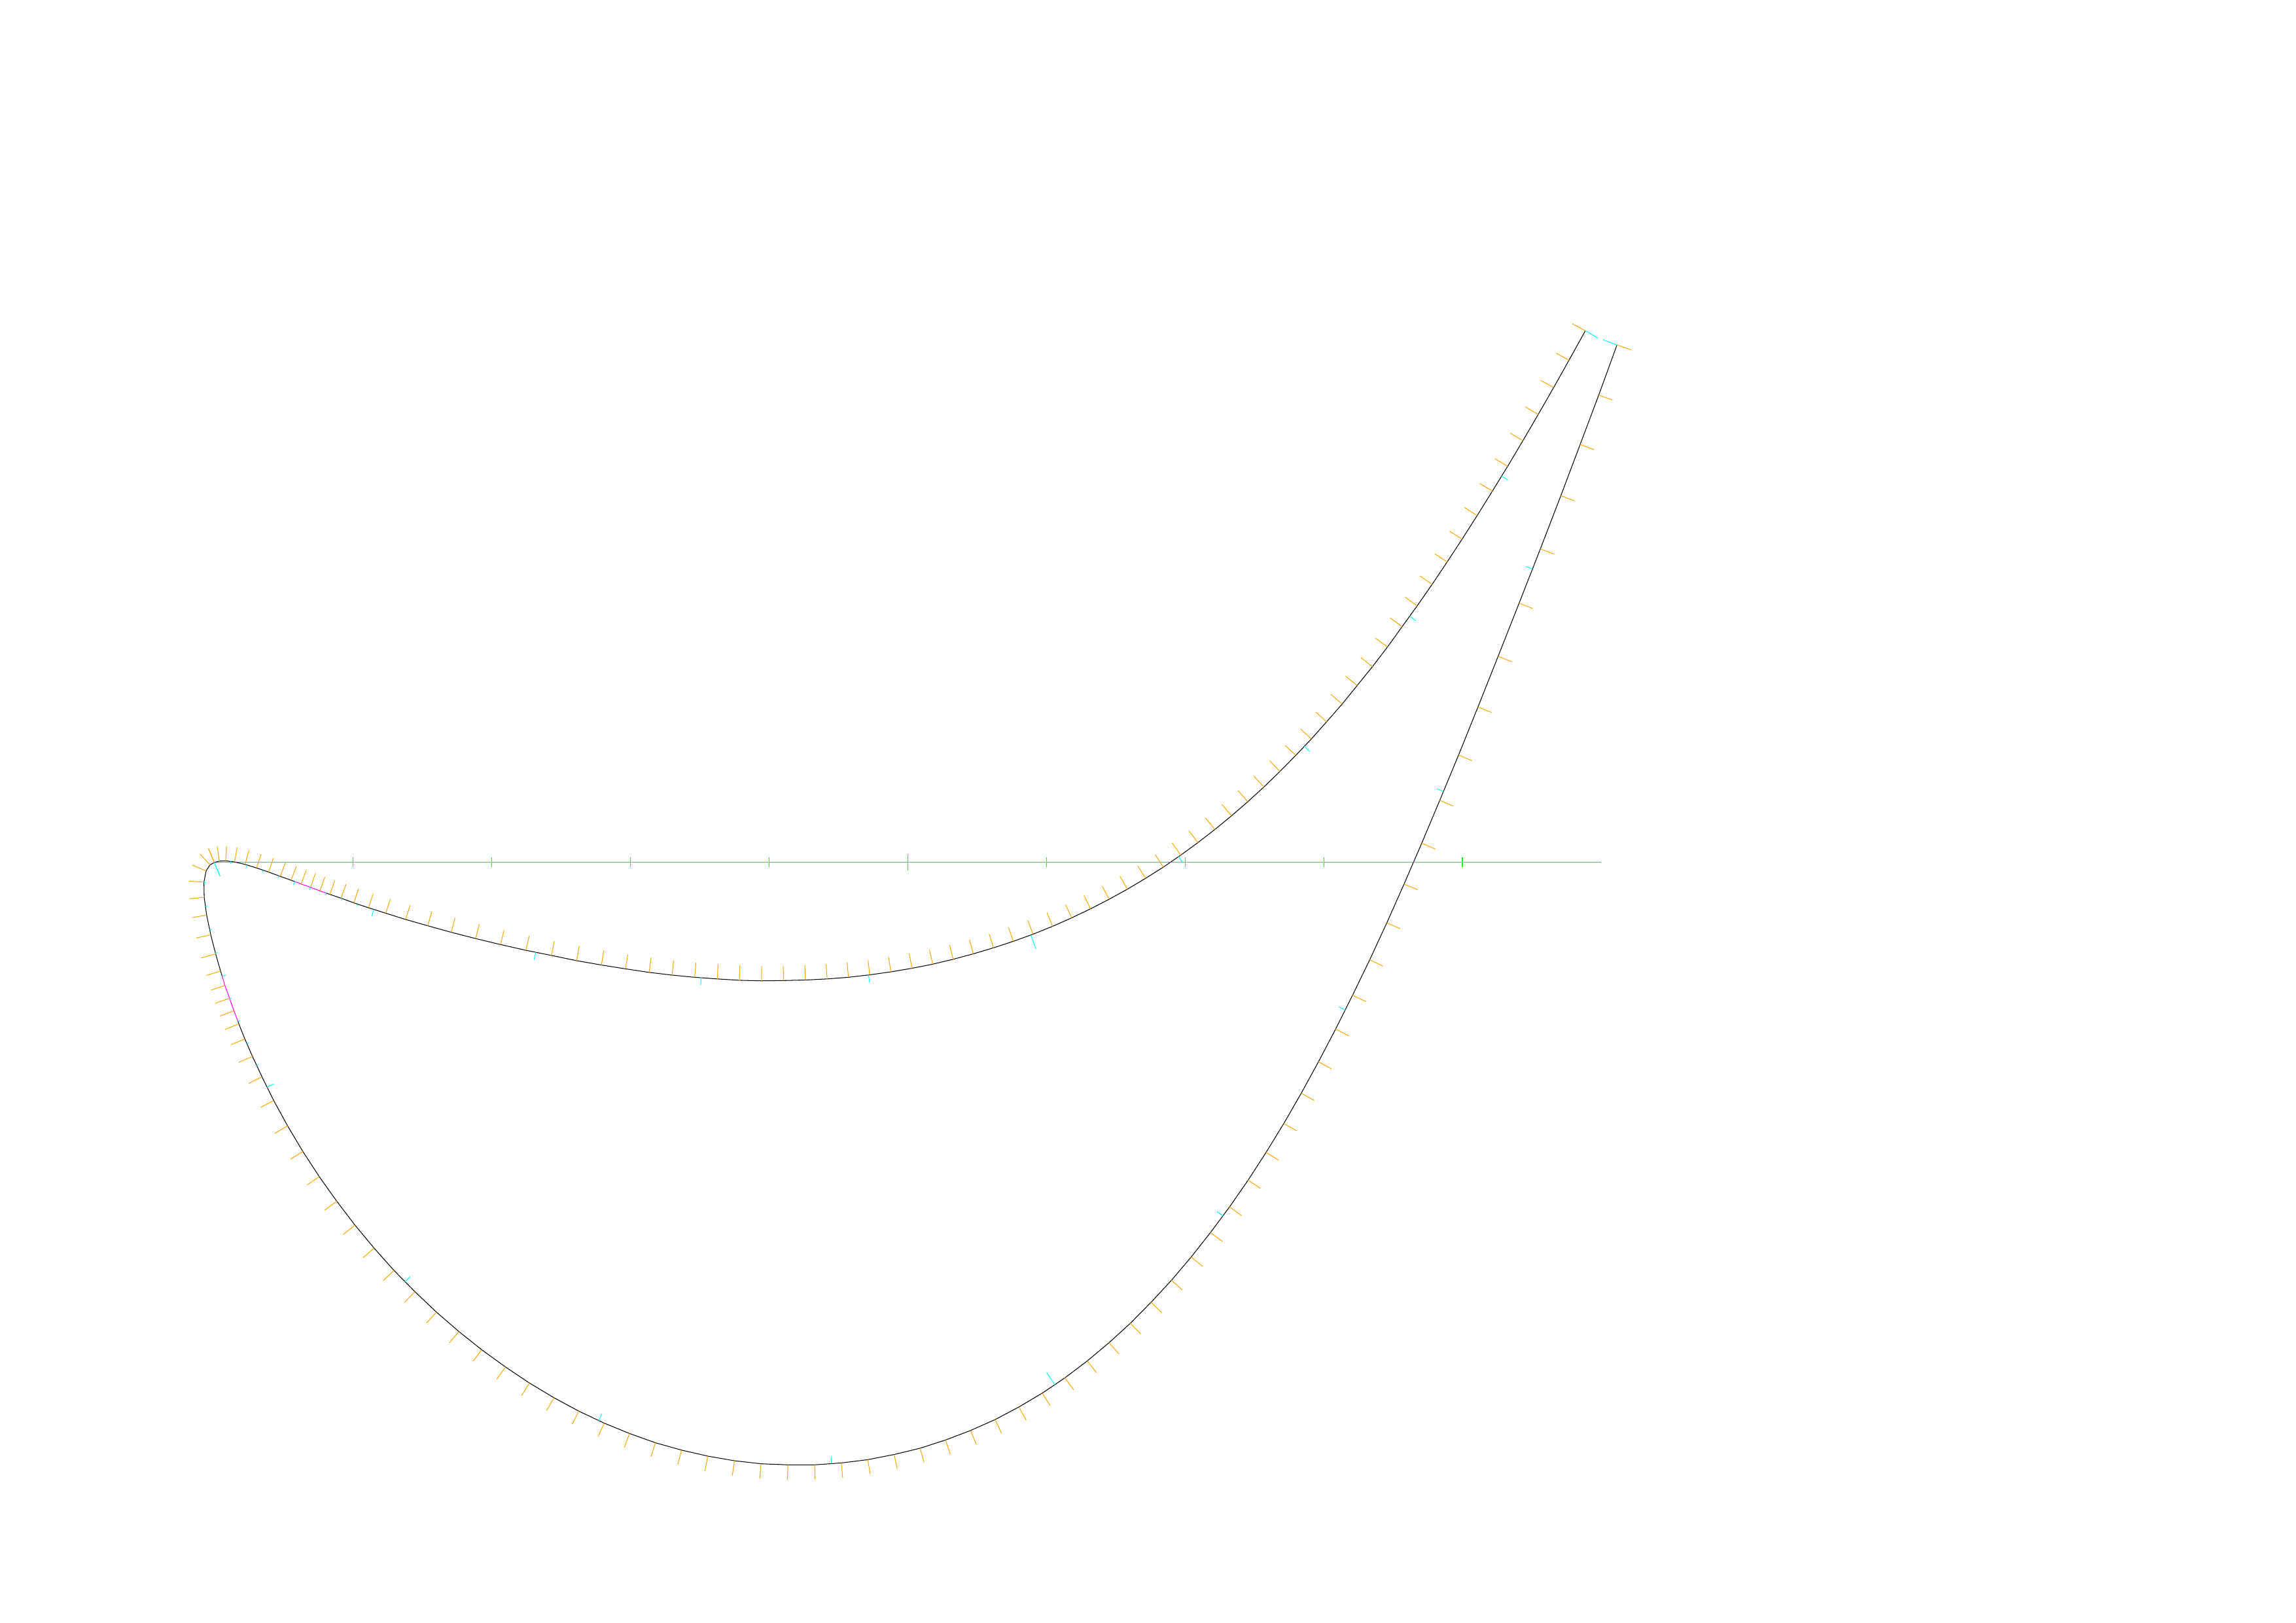
\includegraphics[scale=0.3]{./images/datablade120-2.png}
        \end{figure}
        \column{0.5\textwidth}
        \begin{figure}
            \centering
            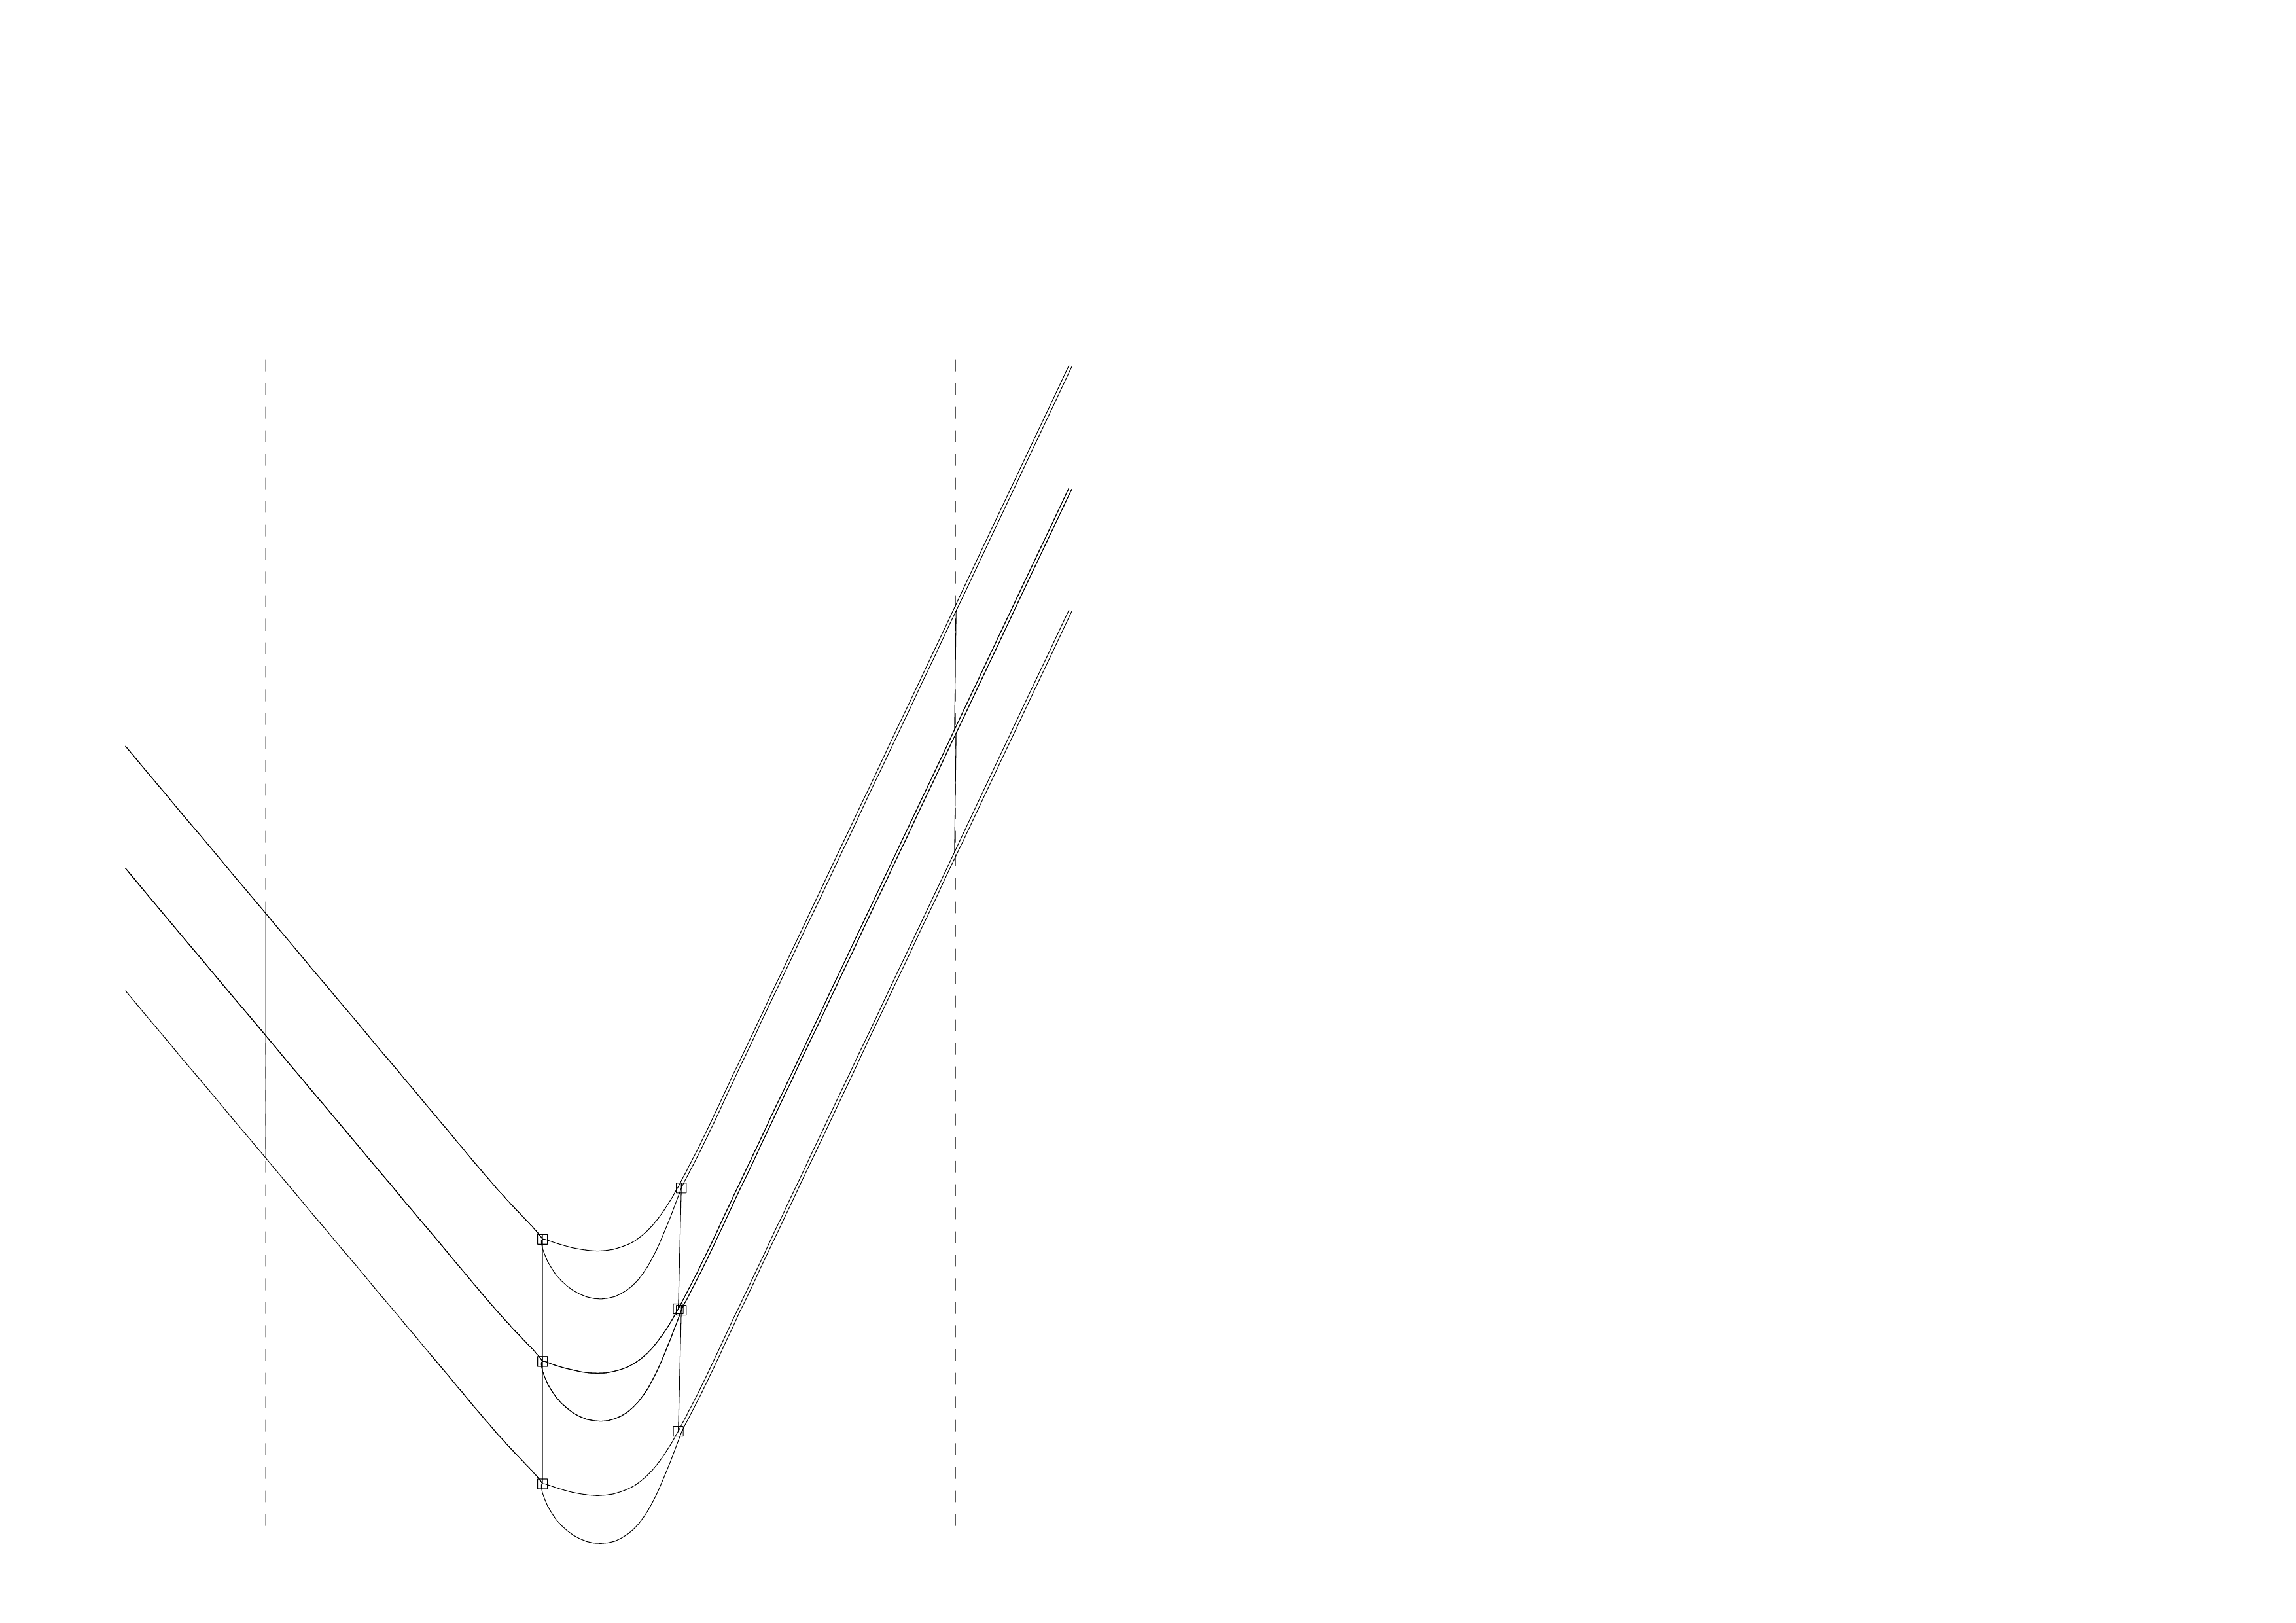
\includegraphics[scale=0.4]{./images/datablade120-1.png}
        \end{figure}
    \end{columns}
\end{frame}

\begin{frame}{\texttt{MISES} - Grid \& flow}
    \vspace{-2.5cm}
    \begin{columns}
        \column{0.5\textwidth}
        \vspace{0.5cm}
        \begin{figure}
            \centering
            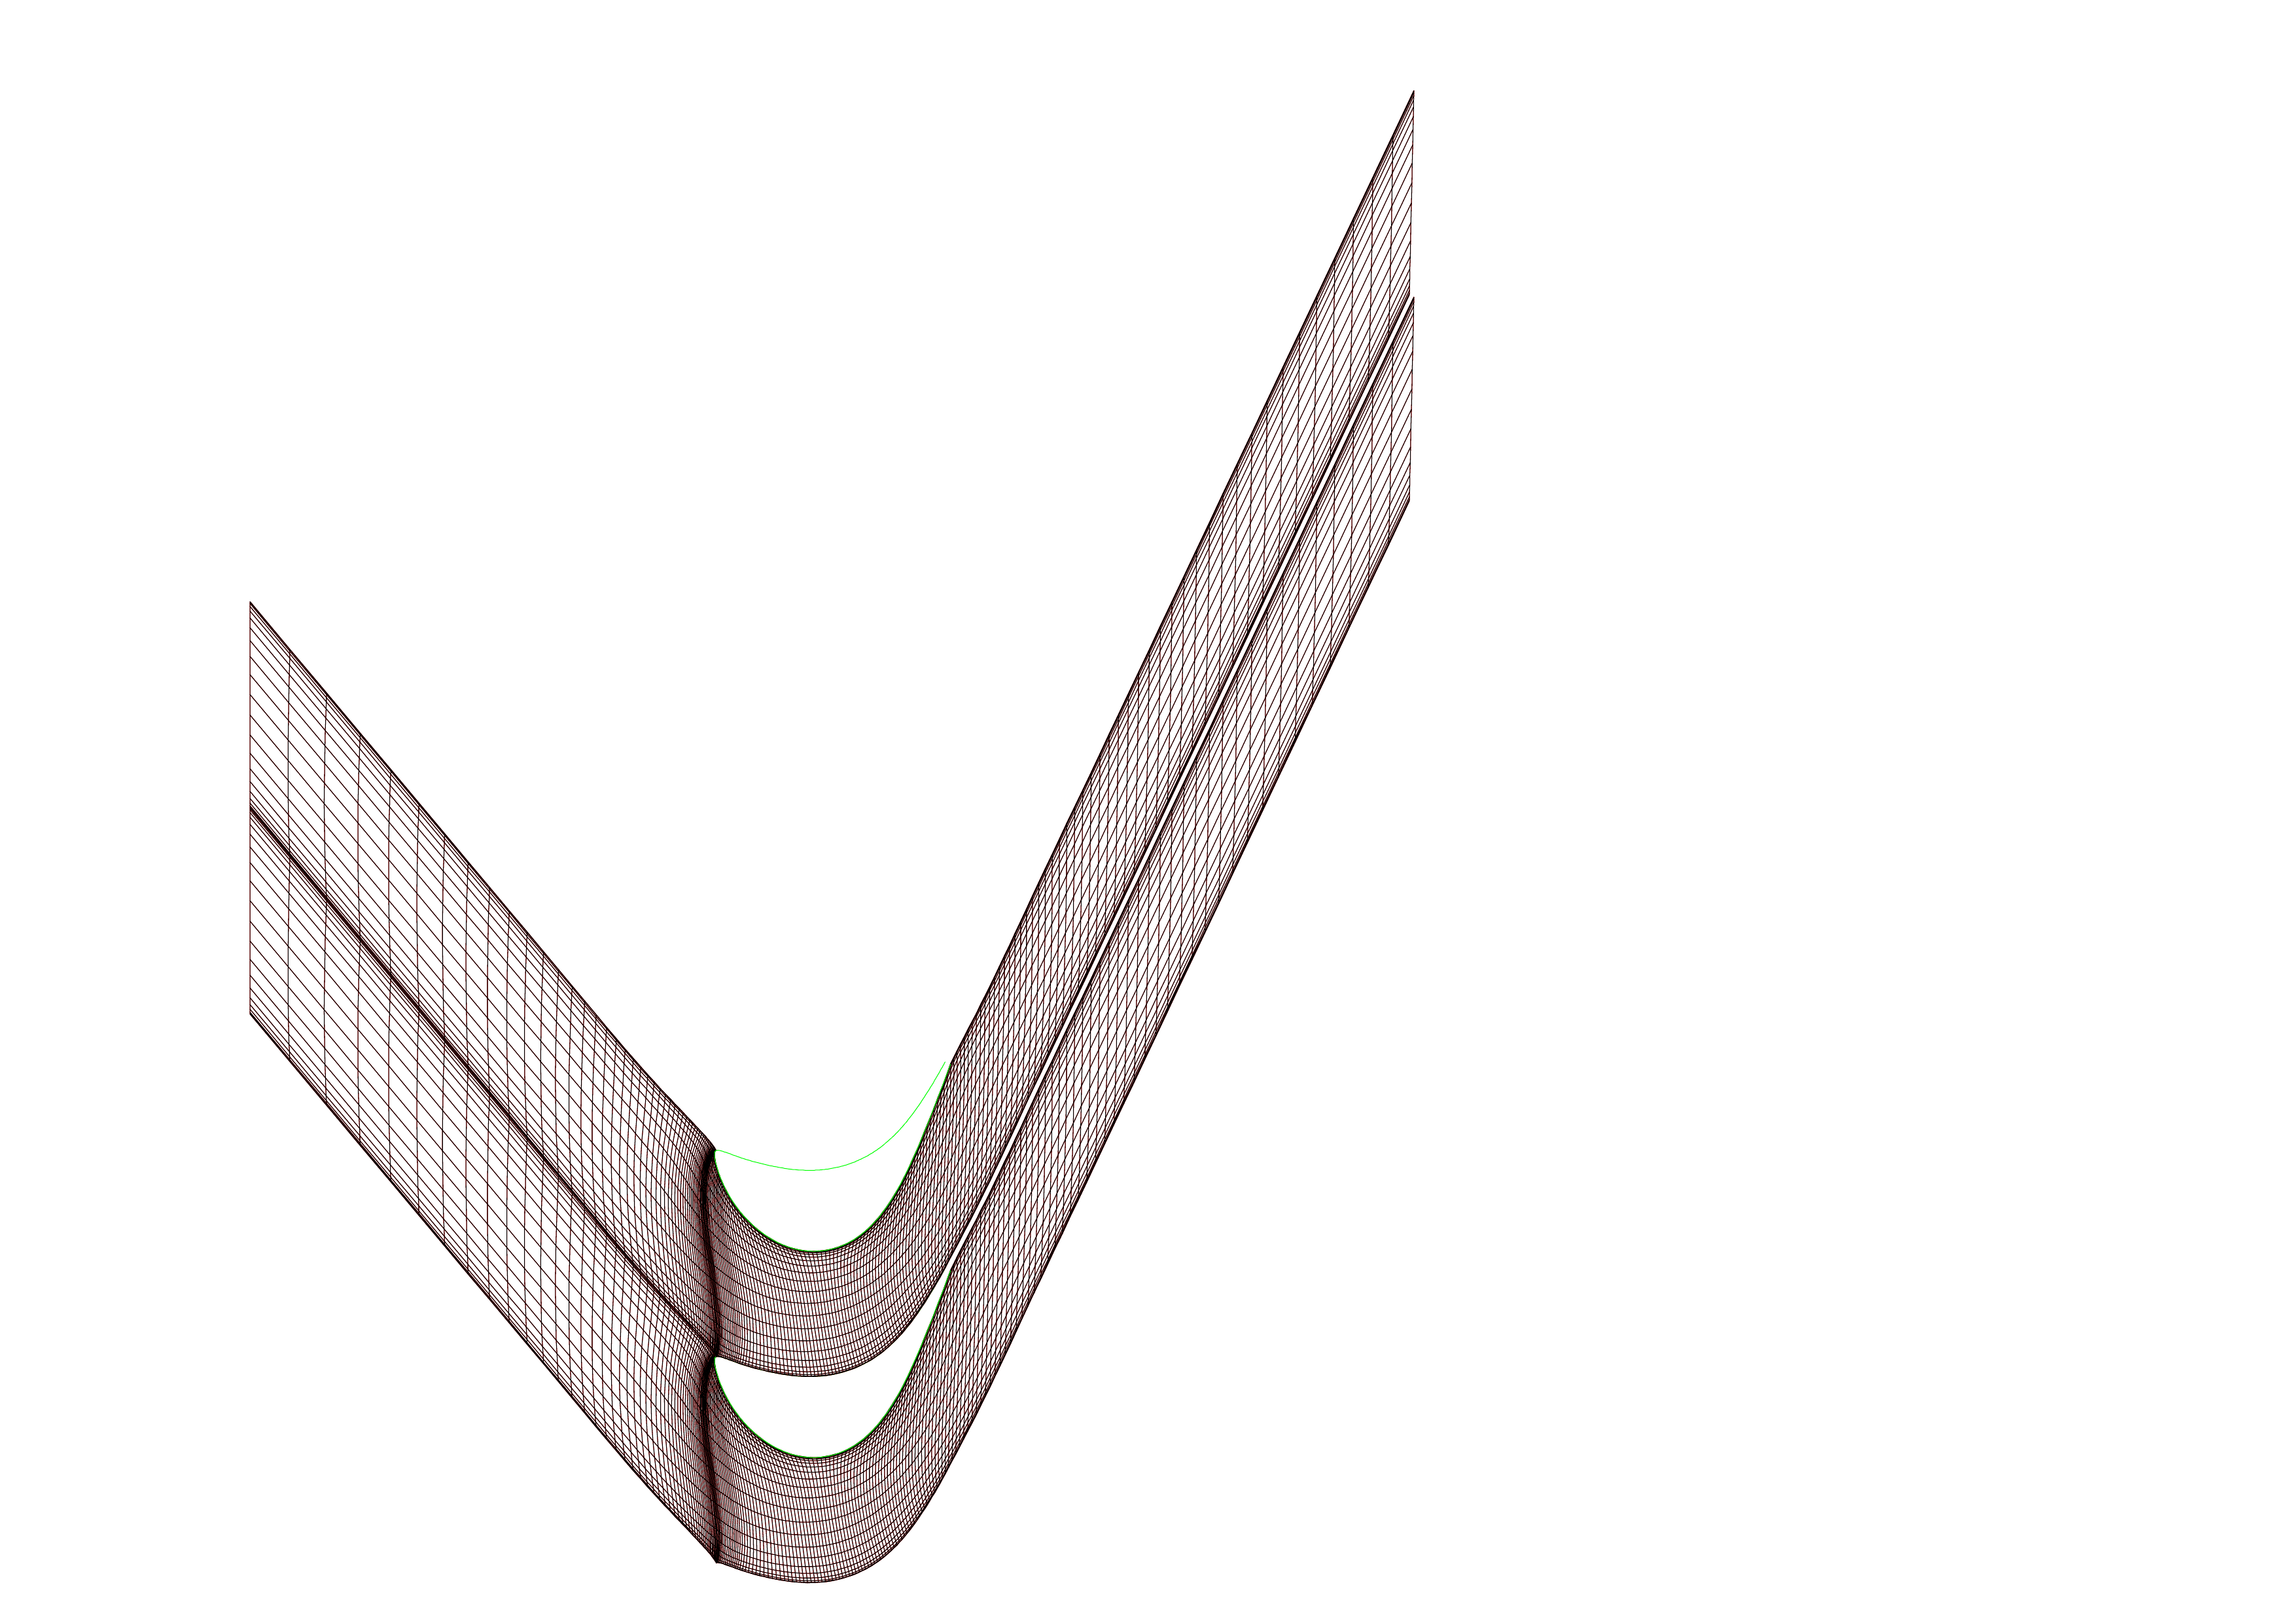
\includegraphics[scale=0.4]{./images/datablade120-3.png}
        \end{figure}
        \column{0.5\textwidth}
        \begin{figure}
            \centering
            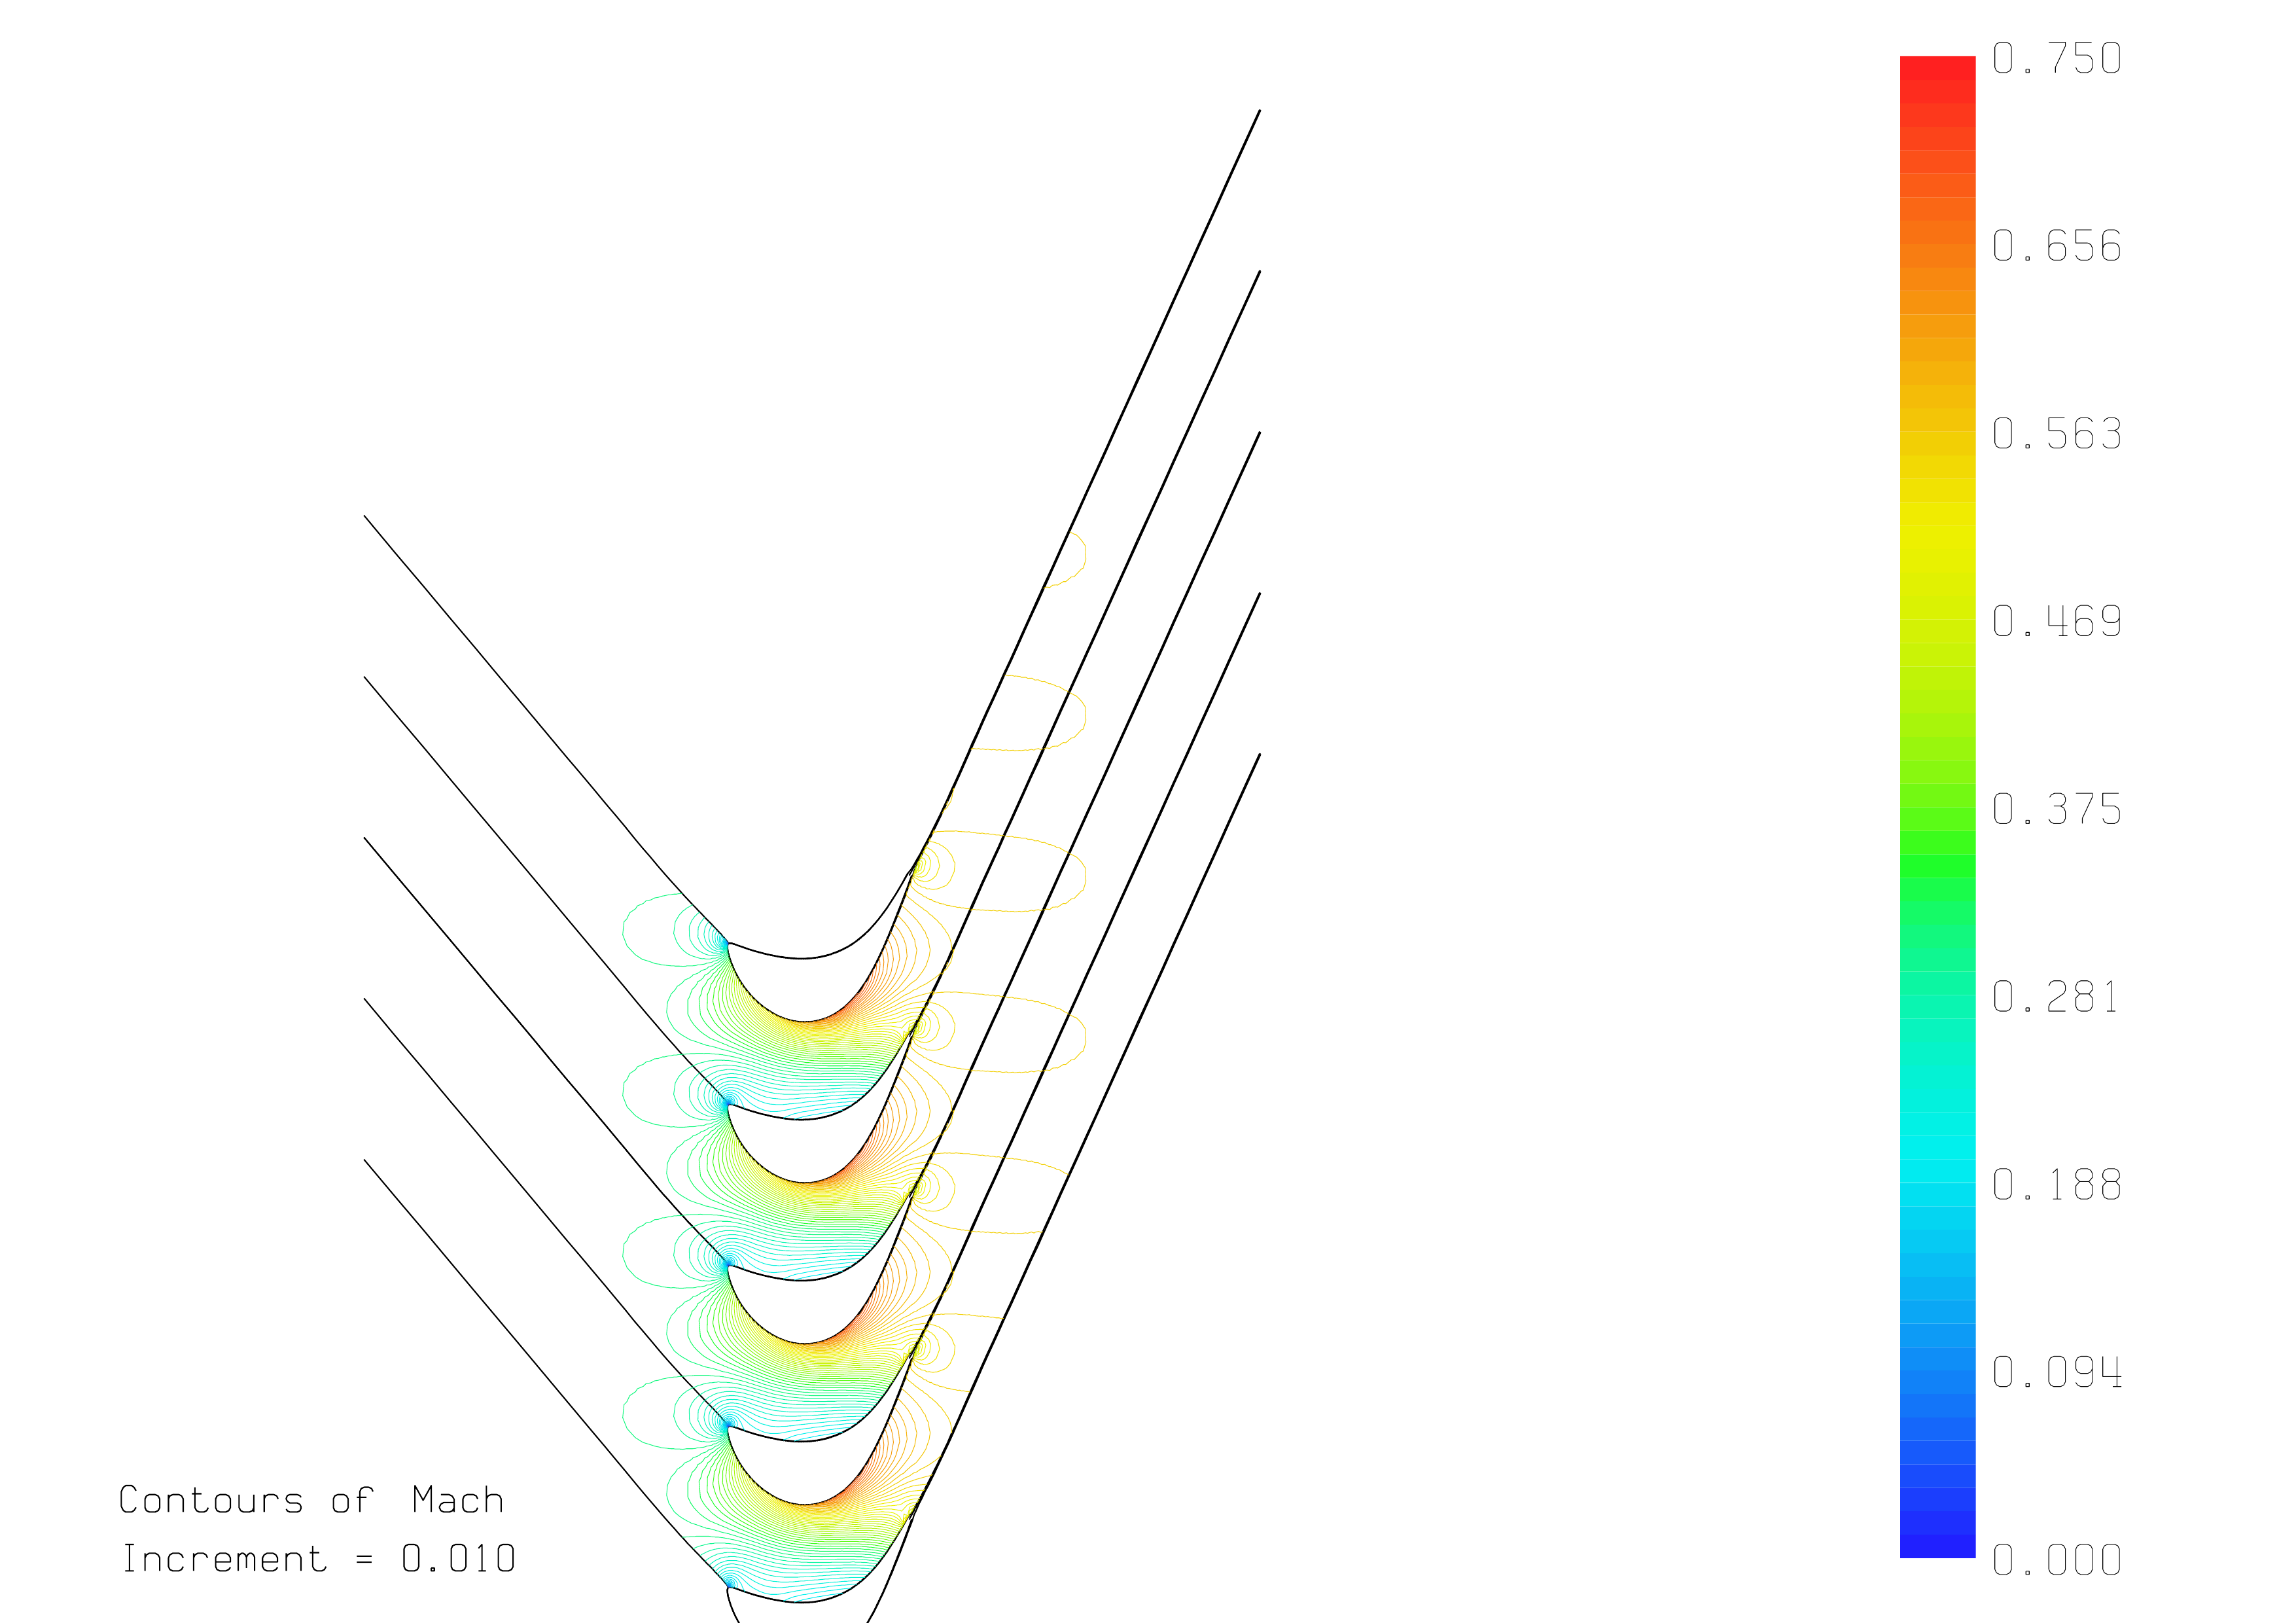
\includegraphics[scale=0.4]{./images/datablade120-4.png}
        \end{figure}
    \end{columns}
\end{frame}

% \begin{frame}{\texttt{MISES} Input -- Setup}
%     \begin{block}{Inputs}
%         \begin{itemize}
%         \item Flow properties:
%         \begin{itemize}
%             \item \texttt{MOUT = } $ M_2$: mixed outlet Mach flow
%             \item \texttt{SINL = } $\tan(\alpha_{1})$: inlet flow angle slope
%         \end{itemize}
%         \item Grid properties:
%         \begin{itemize}     
%             \item \texttt{F F}: grid setup, \texttt{H-type} grid for the inlet, the blade-to-blade plane and the outlet of the mesh
%         \end{itemize}
%         \item Turbulence:
%         \begin{itemize}
%             \item \texttt{REYin = } $Re = 6 \cdot 10^5$: flow Reynolds number
%             \item \texttt{NCRIT = } $n_{crit} = 4$: turbulence model parameter following Abu-Ghannam-Shaw model
%             \item \texttt{XTR1 = XTR2 = } $0.15$: imposed turbulence transition point over the blade
%         \end{itemize}
%     \end{itemize}
%     \end{block}
% \end{frame}

% \begin{frame}{\texttt{MISES} Input -- Properties}
%     \begin{alertblock}{Grid properties and test}
%         After many tests comparing \texttt{H-type} grid with \texttt{I-type} grid. The \texttt{H-type} grid allows faster execution time for the flow computation with neglecting difference on the flow output to \texttt{I-type} based simulations. This because shock waves are not present inside the domain.
%     \end{alertblock}
%     \begin{alertblock}{Turbulence properties}
%         \begin{itemize}
%             \item The $n_{crit}$ parameter has been chosen looking at a \texttt{MISES} input file for a turbine blade that sits in the working range conditions.
%             \item During the simulation, the turbulence model will then adapt the transition points to the most physical positions on the blade. This number is setup for reducing simulation convergence steps.
%         \end{itemize}
%     \end{alertblock}
% \end{frame}

% \begin{frame}{\texttt{MISES} simulation}
%     \begin{block}{Simulation}
%         \begin{itemize}
%             \item \texttt{ISMOM = 4}: this is the setup to attack the problem. The flow is studied as isentropic in the whole system except where shocks are present (which in this range of study are not so common). The switch from one solver to another is dictate by the $\rho$ field.
%             \item Log files are generated after each simulation for convergence tracking and flow properties study.
%             \item Computation of the Mach distribution over the blade.
%         \end{itemize}
%     \end{block}
% \end{frame}

% \hidelogo
% \begin{frame}{Postprocessing}
%     \begin{alertblock}{Load error computation}
%         The steps followed for the error computation on the aerodynamic load are:
%         \begin{itemize}
%             \item \texttt{MISES} computation
%             \item \texttt{MISES} call that generated Mach distribution over the blade
%             \item Reading of the Mach distribution file getting Mach curve and $M_{TE}$ for the Mach fraction generation
%             \item Computation of the RMSE error using the aerodynamic style target and the Mach fraction load converted in surface fraction. 
%             \item Cost computation 
%         \end{itemize}
%     \end{alertblock}
% \end{frame}
% \begin{frame}{Cost Function}
%     The cost function for the optimization of the blade is:
%     \begin{align*}
%         \Delta \alpha_2 & = | \alpha_{2, \texttt{MISES}} - \alpha_2 | \\ 
%         cost            & = RMSE \cdot \big[1 + 0.01 \cdot \big( 2 \cdot max(0, \Delta \alpha_{2} - \alpha_{th}) \big)^2 \big] \notag
%     \end{align*}
%     \begin{itemize}
%         \item The cost function allows to reduce the outlet flow angle error and the error on the load distribution at the same time. 
%         \item $\Delta \alpha_2$ is the absolute value of the error over the exit flow angle.
%         \item The $\alpha_{th}$ value is a threshold on the outlet flow error.
%     \end{itemize}
% \end{frame}

